\chapter{Introduction} \label{chap:introduction}

%==============================================================================================================================
%											Challenges Nuclear Material Design
%==============================================================================================================================	

Over the years, nuclear science and technology has made many positive contributions towards improving the quality-of-life of millions of people. Nuclear provides the world's second-largest source of low-carbon energy but it also helps control the spread of diseases, assists in diagnosis and treatment of cancer, powers space exploration missions, and drives the advancement of industry, agriculture and technology. Nuclear energy is not only at the core of world's sustainable development efforts but is also poised to take on an even bigger role as the world collectively moves to decarbonise many hard-to-abate sectors of the economy. 
%Recent years have seen a rapid shift in the engineering design of materials. Modelling and simulation have become essential tools in this context and are moving towards a multiscale, multiphysics approach where various physical phenomena  are coupled to enhance the accuracy of predictions. Of particular interest in this regard is the increasing desire to couple thermodynamics codes with other multiphysics codes such as phase field, fuel performance codes, etc. This chapter provides a brief background to the proposal and presents the motivation behind the proposed work.

%\section{Introduction}
%	Global population and per capita energy consumption are rising and electrical power generation not only plays a key role in the advancement of industry, agriculture, technology and the quality of living but is also an important measure of a country's economic development, power and independence. The global energy consumption has had significant impact on the environment in terms of greenhouse gas emissions and degradation of the quality of air, water and land.  As the call for action on climate change has become more pronounced and more urgent, there have also been concerns about energy security resource sustainability and human health. This has generated a renewed interest in nuclear energy as a source of reliable, low carbon footprint electricity source.

	As of 2022, around 440 nuclear plants around the world supplied \SI{2653}{\tera\watt\hour} of electricity, around 10\% of the world's total electricity \cite{WNA:2019aa}. Despite the strong support for, and growth in, intermittent renewable electricity sources in recent years, the fossil fuel contribution to power generation has remained virtually unchanged over the last decade and a half \cite{WNA:2019aa}. In its World Energy Outlook 2021, the Organisation for Economic Co-operation and Development (OECD) International Energy Agency (IEA)  has proposed an ambitious \emph{Sustainable Development Scenario} consistent with the goals clean and reliable energy and a reduction of air pollution, among other aims. In the scenario, by year 2050, nuclear based electricity generation should increase by 75\% to \SI{4714}{\tera\watt\hour}, a  capacity growth to \SI{669}{\giga\watt\electric} \cite{IEA:2018aa}. Key to a sustained growth of nuclear power is demonstrating their safety, reliability and economy.
	
	Though many nations across the globe, both industrialised and developing, are confident of the potential of nuclear energy, several challenges related to sustainability, reliability, economic competitiveness, safety, risk of proliferation, anticipated future needs beyonds electricity, and need for government support  remain \cite{GIF:2009aa}. To meet these challenges and develop future nuclear energy systems, the Generation {IV} International Forum (GIF) is undertaking necessary research and development to develop the next generation of innovative nuclear energy systems that can supplement today's nuclear plants and transition nuclear energy into the long term \cite{GIF:2019aa}. While promising in terms of sustainability, economics, safety and reliability, and proliferation resistance and physical protection, the Gen-{IV} nuclear reactors pose unique challenges in terms of engineering design, modelling and construction of these reactors. The design issues are themselves quite complicated and span a wide array of knowledge domains such reactor physics, chemistry, materials science, fluid flow and heat transfer, etc. Safe and economical operation of any nuclear system relies heavily on the success of nuclear fuels and structural materials which must operate under extreme environments. Compared to current generation of reactors, advanced reactors will operate at higher temperatures, under higher irradiation, at higher pressures, and in some cases, like Molten Salt Reactors (MSRs), with fluids that present more challenging corrosion problems \cite{Allen:2010aa}.

	
\section{Material Challenges in Nuclear Systems}

\section{CT in Nuclear}

MSR - Chemistry is very important, fuel salt composition (TC is imp here), corrosion, etc. PIRT Holcomb.

\section{Modelling and Simulation}
	The environment in a nuclear reactor induces complex multiphysics phenomena in nuclear materials, occurring over distances ranging from inter-atomic spacing to meters, and times scales ranging from microseconds to years. This multiphysics behaviour is often tightly coupled and many important aspects are inherently multidimensional  \cite{WILLIAMSON2012149}. Once in the reactor, nuclear materials are subjected to extreme radiation environments that continuously alter their thermo-mechanical properties \cite{STAN200920}. Moreover, due to irradiation effects, the physics and chemistry of such materials become more complicated over time. The safe and reliable performance of nuclear power plants requires choice of suitable materials and the assessment of long-term materials damage.

	Modern materials, including nuclear materials are developed using a combination of discovery, which involves evaluating existing materials to identify candidates with desirable properties, and design, which aims at  creating new materials with predefined qualities \cite{STAN200920}. While the traditional approach to discovery and design of materials was almost entirely experimental, recent developments in modelling and high performance computing has resulted in a much stronger collaboration and integration among theory, experiments and computational science. Multiscale, multiphysics models and simulations enable investigations over  a wide range of length and time scales which would otherwise be unfeasible using only experiments. Thus, computational models help augment and guide experimental campaigns and support economical discovery and design of materials within reasonable lead times.

	With material issues ranging from creep, swelling, fracture, fatigue to corrosion, impurity  effects and correlation between nano and microstructural scale, it is evident that a multiscale approach is required for a fundamental understanding of all the relevant phenomena. However, due to significant limitations on availability of computing resources, a majority of materials modelling and simulation efforts in the past adopted an operator splitting approach wherein the various physical phenomena were disconnected from each other. Though these methods were suitable for previous generation of nuclear reactors, addressing the materials challenges for advanced reactors requires a tightly coupled multiscale, multiphysics approach.

	\begin{figure}[htbp]
		\centering
		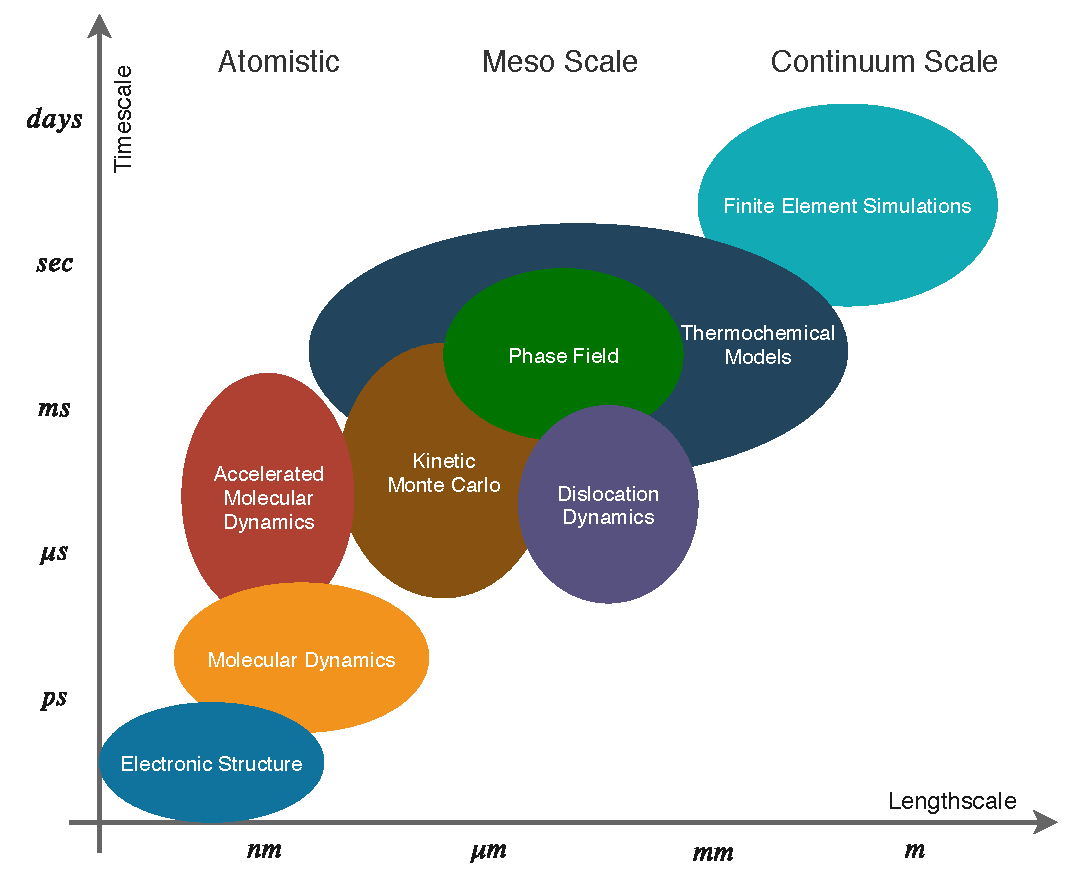
\includegraphics[width=0.75\textwidth]{figures/Multiphysics.pdf}
		\caption{Multiscale theoretical and computational methods used for materials model development and computer simulation \cite{STAN200920}.}
		\label{fig:multiphys}
	\end{figure}

	Traditionally, nuclear material modelling has focussed on the macroscale behaviour of the materials. Such models rely on the principles of thermo-mechanics and are heavily rooted in experimental observations. For example, nuclear fuel behaviour is often modelled as a solid mechanics problem coupled with conductive heat transfer and fission gas release wherein the material properties are often either assumed to be constant or described using simplified models based on empirical correlations. Recently, there has been an impetus on atomistically informing mesoscale  and macroscale methods by optimising characteristic parameters of these scales against the output of atomistic calculations \cite{STAN200920}. Since such an approach is rooted in fundamental principles, the transfer of information between scales, through characteristic parameters such as density, energy, temperature, etc., results in a much more accurate description of material behaviour. Some of the theoretical and computational methods used in multiscale approach have been shown in figure~\ref{fig:multiphys}.

	\subsection{Corrosion in materials}
	Many emerging nuclear technologies, such as the Molten Salt Reactors (MSR), use high temperature fluids, such as molten fluoride/chloride salts, which lead to corrosion of the metal containment leading to problematic behaviours during the reactor operations. Corrosion in molten salts is a fundamentally different process from that in conventional applications, and most of the methods to control corrosion developed over previous centuries are of limited value \cite{Yoshioka:2017aa}. In fluoride salts, the protective oxide layer on alloys typically relied upon for high-temperature corrosion resistance dissolves, thereby exposing the fresh alloy surface to the molten salt. In molten chloride salts, passivity has been observed; however, the oxide layer is prone to attack and may not provide the necessary corrosion protection \cite{Sridharan:2013aa}. The corrosion process is accelerated by the impurities present in the salt and enhanced further by the presence of dissimilar metals due to activity-driven corrosion. Another issue to be considered is the mass transfer of corrosion products from hotter sections of the nuclear reactor and subsequent deposition in the colder areas that can clog the heat exchanger systems. Therefore, effectively predicting corrosion and related phenomena like leaching and deposition requires a multiscale, multiphysics approach \cite{Mcmurray:2018aa}.

	Corrosion is an electrochemical process composed of oxidation and reduction reactions, which are defined by the thermodynamics and kinetics of the system. While thermodynamics controls whether or not a material may corrode, kinetics influences how quickly the material will corrode. This corrosion behaviour is also significantly affected by the material microstructure and predicting corrosion therefore requires a multiphysics approach that can couple quantitative electrochemistry models of corrosion and chemical reactions with thermochemical equilibrium computations.

	\subsection{Thermodynamic modelling of materials}
	The phase and chemical behaviour of nuclear materials is governed by the thermochemical equilibrium state. While in many systems, equilibrium is often not achieved due to transport and/or chemical kinetics phenomenon, a thorough understanding of both transport and chemical evolution, and subsequently material properties, is  based on an accurate representation of thermochemical equilibria \cite{Devanathan:2010aa}. As an example, the oxygen chemical potential acts as the driving force for transport of oxygen in oxide fuels but a determination of these chemical potentials is impossible without determining the stable phases which depends on the oxygen-to-metal ratio which in turn is a function of burnup.  In the specific context of corrosion modelling, the difference in the free energy of the salt fluoride/chloride constituents and the fluorides/chlorides of the alloying elements is a key driving force for corrosion. For closed systems, the equilibrium concentration of the corrosion product fluorides/chlorides in the salt melt dictates the maximum extent of corrosion and is important in the long-term corrosion of containment materials. Therefore, thermodynamic equilibrium calculations play an important role in the context of corrosion modelling in advanced reactors.

	Capturing thermodynamic equilibria in multiphysics codes has traditionally relied on empirical correlations and the interest in direct coupling of thermodynamic equilibrium codes with multiphysics model is only a recent trend. While the empirical correlations do not convey the high fidelity of original thermodynamic analysis, performing thermodynamic equilibrium analysis within multiphysics codes is normally a very complex process and can significantly impede the computational performance of such codes. However, the recent developments in high performance computing have enabled the incorporation of these calculations which are of ever more importance in the discovery and design of materials for advanced reactors.

	The inputs for a thermodynamic equilibrium calculation are shown in figure~\ref{fig:Thermod}. Since thermodynamic equilibriums are isothermal and isobaric in nature, temperature and pressure are required as inputs along with the elemental composition of the material. While the equilibrium calculations are mathematically rigorous they do require thermodynamic models of materials to describe some parameters.  These thermodynamic models are generally developed using the Calculation of Phase Diagram (CALPHAD) approach shown in figure~\ref{fig:calphad}, which combines experimental and theoretical information to describe the thermodynamic properties through the Gibbs energy, applying a mathematical model containing adjustable parameters \cite{Lukas07}.  The multiscale approach also allows \textit{ab initio} molecular dynamics calculations to inform and improvise the thermodynamic models developed using the CALPHAD approach.
	\begin{figure}
        		\centering
        		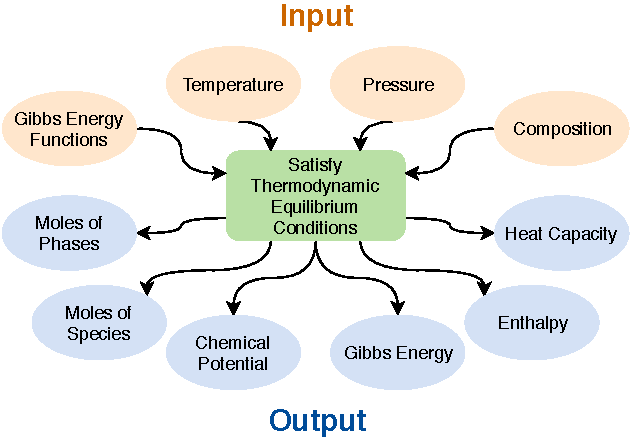
\includegraphics[width=0.75\textwidth]{figures/Thermodynamics.pdf}
        		\caption{Input and output parameters of thermodynamic equilibrium calculations.}
        		\label{fig:Thermod}
    	\end{figure}

Figure~\ref{fig:Thermod} also shows some of the outputs produced by thermodynamic equilibrium calculations. The main outputs include the phase assemblage, i.e. the number of moles of phases present at equilibrium and the mole fraction of the species in those phases. The equilibrium calculations also provide the Gibbs energy of the system, the chemical potentials of the species, etc. These quantities are useful in multiphysics calculations where, for example, the chemical potential of oxygen can be used to model oxygen diffusion in a \ce{UO2} nuclear fuel pellet.
	\begin{figure}[htbp]
	\centering
	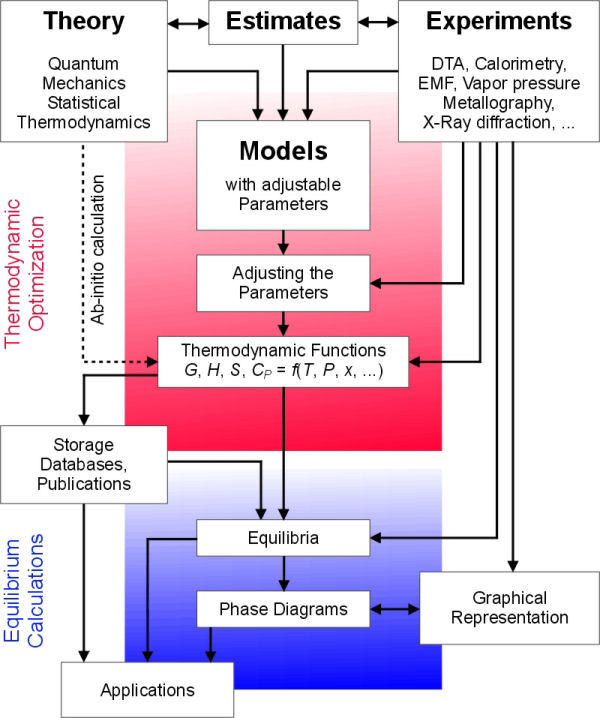
\includegraphics[width=0.5\textwidth]{figures/Calphad_method}
	\caption{Principle of CALPHAD method by Zinkevich \cite{Zinkevich:2003aa}}
	\label{fig:calphad}
	\end{figure}

\section{Multiphysics Object Oriented Simulation Environment}
	The  Multiphysics Object-Oriented Simulation Environment \texttt{(MOOSE)} is a tool for solving complex coupled multiphysics equations using the finite element method. \texttt{MOOSE} uses an object-oriented design to abstract data structure management, parallelism, threading and compiling while providing an easy to use interface targeted at engineers that may not have a lot of software development experience. \texttt{MOOSE} provides extreme scalability and flexibility when compared to other finite element method (FEM) frameworks. For instance, \texttt{MOOSE} has the ability to run extremely complex material models, or even third-party applications within a parallel simulation without sacrificing parallelism. This capability is in contrast to what is often seen in commercial packages, where custom material models can limit the parallel scalability, forcing serial runs in the most severe cases \cite{gaston2015physics,moose-web-page}.

	The design goal of \texttt{MOOSE} is to give developers ultimate control over their physical models and applications. Designing new models or solving completely new classes of problems is accomplished by writing standard C++ source code within the framework's class hierarchy. Scientists and engineers are free to implement completely new algorithms using pieces of the framework where possible, and extending the framework's capabilities where it makes sense to do so. Commercial softwares do not have this capability, and instead opt for either a more rigid parameter system or a limited application-specific metalanguage \cite{moose-web-page}.

	Currently, apart from a number of other applications, such as \texttt{RELAP} \cite{Zhang:aa} for system level thermal hydraulics, \texttt{Rattlesnake} \cite{Wang:aa} for neutronics, etc., the \texttt{MOOSE} framework consists of two main applications for materials applications - the macroscale fuel performance code \texttt{Bison} \cite{Newman09} and the mesoscale phase field code \texttt{Marmot}  \cite{Tonks12}. Together, \texttt{MOOSE}, \texttt{Bison}  and \texttt{Marmot}, form the Fuels Product Line (FPL) to deliver an integrated set of increasingly predictive computational tools for nuclear fuel performance analysis and design. The FPL enable multiscale modelling and simulation of nuclear fuels where simulations of fuel performance at the engineering scale are informed by material property and behaviour models developed from mesoscale simulations of microstructure evolution under irradiation, which are themselves guided and enabled by inputs of fundamental materials parameters obtained from atomistic simulations. The multiscale, multiphysics approach allows an unprecedented degree of predictability of nuclear fuel performance.

	\subsection{Bison}
	The simulation of nuclear reactor fuel performance involves complex thermomechanical processes between fuel pellets, made of fissile material, and the protective cladding barrier that surrounds the pellets. \texttt{Bison} is an engineering scale code developed to predict the nuclear fuel performance under normal, off-normal, and accident conditions. By using highly efficient computational methods, \texttt{Bison} enables three dimensional, fully coupled multiphysics simulations on high fidelity geometric representations of fuel pins/pellets. \texttt{Bison} has been designed to be highly scalable and does not require the use of operator splitting, staggered or predictor-corrector approaches \cite{WILLIAMSON2012149}.

	Within the multiscale framework, \texttt{Bison} can be coupled with both mesoscale microstructure evolution tool \texttt{Marmot} as well as reactor core and system tools being developed under the Reactor Products Line to perform full scale simulations of the entire nuclear reactor. Coupling with \texttt{Marmot} allows \texttt{Bison} to easily and continuously incorporate new mechanistic, physics-based models produced by the mesoscale model development activities in order to extend its predictive capability to new fuels and operational regimes. While focussed on Light Water reactor (LWR) fuel, \texttt{Bison} is applicable to variety of fuel forms including the spherical TRISO fuel design \cite{NEAMS}.

	\subsection{Marmot}
	Due to its simple concept and large range of applicability, the phase field approach is a popular and powerful tool to model microstructure and has been applied in problems such as grain boundary migrations, martinistic transformation, two-phase flow, etc. The phase field approach treats all material interfaces as diffuse by representing structural features with continuous variables which smoothly transition from one value to another. Thus, phase field method not only eliminates the need to explicitly discretise boundaries and interfaces, it also enables describing microstructure through a system of partial differential equations.  The \texttt{Marmot} phase field framework has been developed to enable simulations of the microstructure evolution of nuclear fuels and materials under irradiation. By exploiting the object-oriented architecture of \texttt{MOOSE}, \texttt{Marmot} allows easy coupling of phase field with additional physics such as solid mechanics or heat conduction, to effectively predict the microstructural evolution at mesoscale. This allows prediction of evolution of material properties of nuclear materials under irradiation and can be used to inform engineering scale simulations and reduce the dependence of such simulations on empirical correlations. As a result, the multiscale framework can achieve true predictability even in compositional and operational regimes where little or no experimental data exists.

	Despite the wide ranging capabilities of the FPL, there remains a gap in terms of modelling advanced nuclear reactors. The high temperature operations of reactors such as the Molten Salt Reactors (MSR), which use molten fluoride/chloride salts as the fuel and coolant, produce a conducive environment for corrosion. The current FPL lacks a tool for corrosion modelling at microstructure scale and efforts are underway to develop a new \texttt{MOOSE} based application called \texttt{Yellowjacket} to bridge this gap.

	\subsection{Yellowjacket}
	\texttt{Yellowjacket} is a mesoscale framework for thermodynamics based modelling of corrosion in advanced reactor materials. Currently under development, it is a \texttt{MOOSE} based application that couples quantitative models of corrosion with thermodynamic equilibrium and chemical kinetics models to predict the rate of material loss, corrosion product production and precipitate production in advanced nuclear reactors. \texttt{Yellowjacket} relies on phase field models for structure evolution, coupling it with Poisson equation for electrostatics, fracture models and thermochemical equilibrium solvers to provide a holistic environment for corrosion modelling and simulation. As shown in figure~\ref{fig:yjmoose}, \texttt{Yellowjacket} depends on the \texttt{MOOSE} framework for the development infrastructure and follows the Nuclear Quality Assurance Level 1 (NQA 1) \cite{NQA-web-page} development process.

	\begin{figure}[htbp]
		\centering
		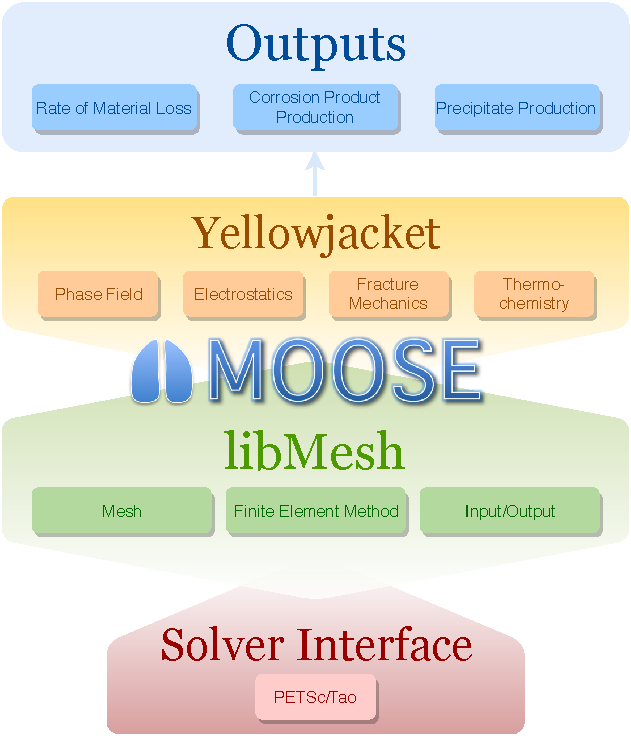
\includegraphics[width=0.75\textwidth]{figures/Yellowjacket_MOOSE.pdf}
		\caption{Illustration showing the underlying interface provided by \texttt{MOOSE} and the physics modules of \texttt{Yellowjacket}.}
		\label{fig:yjmoose}
	\end{figure}

	\texttt{Yellowjacket} is being developed through a joint collaboration between the Nuclear Fuels and Materials Group at Ontario Tech University, University of Florida, Idaho National Laboratory and Los Alamos National Laboratory, and is funded primarily by the United States Department of Energy (US-DOE) through the Nuclear Energy Advanced Modelling and Simulation (NEAMS) program.

	This thesis is aimed at developing a thermodynamic equilibrium solver for the corrosion modelling tool \texttt{Yellowjacket} and the goals of this research are specified in the following chapter. The phase field component of \texttt{Yellowjacket} is being investigated by another PhD student at University of Florida.
